\documentclass{article}

\usepackage{amsmath}
\usepackage{amssymb}
\usepackage{bm}
\usepackage{graphicx}
\usepackage[linesnumbered, lined, boxed]{algorithm2e}
\RestyleAlgo{boxruled}

\DeclareMathOperator*{\argmax}{argmax}
\DeclareMathOperator*{\argmin}{argmin}

\usepackage[citestyle=authoryear]{biblatex}
\addbibresource{paper.bib}

\author{Tom Wallace}

\title{STAT 672 Final Project:\\ Stochastic Gradient Descent}

\begin{document}

\maketitle

\section{Introduction}

\subsection{Organization}

This paper is divided into four sections. The remainder of this
\textbf{Introduction} section gives intuitive motivation for stochastic gradient
descent (SGD). The \textbf{Method and Theory} section more rigorously presents the
mathematics of SGD and some of its notable properties. The
\textbf{Applications} sections highlights the real-world settings and uses of SGD,
including a case study data analysis. The \textbf{Conclusion} section summarizes
overall findings.

\subsection{Motivation}

Optimization is fundamental to statistical modeling. The chief task of
statistical modeling is to characterize the relationship between 
explanatory variables and an outcome variable, and the chief method for doing so
is to estimate values for coefficients that best relate
each explanatory variable to the outcome variable. The term ``best''
implies picking coefficient values that
maximize some measure of goodness (e.g. likelihood) or minimize some measure of
badness (e.g. loss function). 
Mathematical optimization is the typical
route to achieving such minimization or maximization. Two important
considerations for optimization are parametric assumptions and computational
complexity. SGD, an optimization technique, is
particularly motivated by these considerations.

\subsubsection{Parametric vs. non-parametric}

Assuming that the outcome variable follows a
particular statistical distribution aids the computation of optimal coefficients. 
For example, assumptions in ordinary least squares (OLS)
regression---assumptions that readers almost certainly are familiar with and so will not be
repeated here---allow a closed form solution. The optimization problem of
choosing coefficient $\hat{\bm{\beta}}$ that minimize squared error is solved
by $\hat{\bm{\beta}} = (\bm{X}'\bm{X})^{-1}\bm{X}'\bm{Y}$ (where $\bm{X}$ is the
feature matrix and $\bm{Y}$ the outcome variable).

Even if a parametric model does not have a closed-form solution, the parametric
assumption allows some useful optimization techniques. Consider logistic
regression. The maximum likelihood estimator (MLE) approach for estimating
coefficients leads to a system of $D$ equations. This system of
equations typically is numerically solved using the iterative Newton-Raphson
algorithm:

$$
\hat{\bm{\beta}}_{n+1} = \hat{\bm{\beta}}_{n} -
\bm{H}^{-1}(\hat{\bm{\beta}}_n)\bm{J}(\hat{\bm{\beta}}_n)
$$

$\bm{J}$ is the Jacobian (the
first derivative of the log-likelihood function $l$ with respect to each $w_j$)
and $\bm{H}$ is the Hessian (the second derivative of $l$ with respect to $w_j,
w_{j'}$). The practicality of Newton-Raphson thus depends on whether it is convenient to
find $\bm{J}$ and $\bm{H}$. It is convenient for logistic regression
because parametric and independent-and-identically-distributed (IID) assumptions
mean $l$ is a simple sum of the log probability distribution
function (PDF, in this case binomial) for each observation. We ``know'' (assume)
the form of this PDF and so are
confident that the second derivative exists and is not too onerous to calculate.
In non-parametric settings, we often cannot be so certain and face the possibility of
$\bm{H}$ being non-existent or cumbersome.

The need to conduct optimization in non-parametric settings is a chief
motivation for gradient descent (GD), of which SGD is a variant. In
non-parametric settings---most notably supervised and unsupervised statistical
learning, in which we again seek to find optimal coefficients to relate input
variables to output variables for the purposes of classification or regression---there 
typically is no closed form solution for the coefficients. It
also may not be convenient to find and evaluate the Hessian, making
Newton-Raphson undesirable. SGD does not require any parametric assumptions. 
In its most basic form, SGD only requires finding the gradient (though some extensions
do need the Hessian or an approximation to it). 
SGD thus is well-suited for non-parametric settings.

\subsubsection{Computational Complexity}

How an optimization technique scales with sample size $n$ is another important
consideration. It is little comfort if a method reaches the correct solution but
requires an excessive amount of time to do so. ``Plain'' or
``batch'' GD requires evaluating the gradient for every single observation,
every single iteration, until the algorithm converges. For example, for a
dataset of $n=10^6$ that required 25 iterations to converge, batch GD would require 
evaluating the gradient $25 \times 10^6$ times. This scaling with
$n$ can cause untenably long computation time.

SGD alleviates these computational difficulties by requiring the gradient to be
evaluated for only a single randomly chosen observation per iteration. This
approach means convergence is ``noisier'' and hence requires more iterations to
converge, but each iteration is less complex to compute and so can be done
faster. SGD thus scales much more favorably with $n$ than GD, and so is
particularly useful for large-$n$ applications such as machine learning
and big data problems.

\section{Method and Theory}

\subsection{Basic Form}

This section presents the basic form of GD and SGD to set up a more detailed
examination in subsequent sections. Suppose we want to minimize a function $f: \mathbb{R}^D \to \mathbb{R}$. 

\begin{equation}
	\min_w f(w)
\end{equation}

$f$ takes as input $w \in \mathbb{R}^D$. Assume
that $f$ is convex and differentiable, i.e. we can compute its gradient with
respect to $w$, $\nabla f(w)$. The optimal $w$, i.e. that which minimizes (1),
is denoted $\hat{w}$. The iterative GD algorithm for finding $\hat{w}$ is:

\begin{equation}
	w^{(t+1)} = w^{(t)} - \gamma \nabla f(w^{(t)})
\end{equation}

$t$ refers to a particular iteration. Assume that we have supplied an initial
starting guess for $w$ for $t=0$, $w^{(0)}$. $\gamma$ refers to step size (also called
learning rate). Assume for now that $\gamma$ is fixed. The GD algorithm iterates
until some stop condition is met. This may be a fixed number of iterations, or
that the quality of approximation meets some predefined threshold. 
A common stopping condition is when the L2 norm of the gradient
is less than some arbitrarily small constant. 

\begin{equation}
	||\nabla f(w^{(t)})||_2 \leq \epsilon
\end{equation}

Consider a modified situation. Suppose $f$ now takes two arguments, $w$ and $X
\in \mathbb{R}^D$. $f : \mathbb{R}^D \times \mathbb{R}^D \rightarrow
\mathbb{R}$. We have $n$ observations of $X$, and denote by
$\bm{X}_{n \times D}$ the matrix of these observations, with $X_i$ being a
particular observation or row in that matrix. We apply
$f$ over all observations, i.e. $\frac{1}{n} \sum_{i=1}^n f(w, X_i)$. Our new
problem is:

\begin{equation}
	\min_w  \frac{1}{n} \sum_{i=1}^n f(w, X_i)
\end{equation}

We could apply the GD algorithm above to find the optimal $w$.

\begin{equation}
	w^{(t+1)} = w^{(t)} - \gamma \frac{1}{n} \sum_{i=1}^n \nabla f(w^{(t)},
	X_i)
\end{equation}

But, note that doing so requires evaluating the gradient at every single
observation $i \leq n$. This may be computationally intractable for large $n$
and high-dimensional $D$. The innovation of SGD is to instead evaluate only a
single randomly-chosen $i$ at each iteration $t$.

\begin{equation}
	w^{(t+1)} = w^{(t)} - \gamma \nabla f(w^{(t)}, X_i)
\end{equation}

As it turns out, SGD converges to $\hat{w}$ and does so in a computationally
advantageous way compared to GD.

\subsection{Key Properties}

\subsubsection{Correctness}

This section gives both intuition and (partial) proof for why (S)GD converges to
$\hat{w}$.

Intuitively, our assumption that $f$ is convex means that there is one critical
point and it is the global minimum. Basic calculus tells us that this critical
point is located where $f'=0$ (in one dimension) or $\nabla f = 0$ (in higher
dimensions). So our task is to search in the space of $f$ for that point. We
start with some initial guess $w^{(0)}$, and every iteration, move ``down'' the
gradient in search of zero. Every iteration, we check if the gradient is equal
to 0; if not, we keep moving ``down.'' If the gradient is arbitrarily close to
zero, then we have found the critical point, which must be the value of $w$ that
minimizes $f$ and hence is $\hat{w}$ (or at least a close approximation to it).

For a more formal proof---following that of \cite{tibs_notes}---assume (in addition to previously stated assumptions
that $f$ is convex and differentiable) that the gradient of $f$ is Lipschitz-continuous
with constant $L$, i.e. that $||\nabla f(x) - \nabla f(y)||_2 \leq L||x-y||_2$
for any $x, y$. This implies that $\nabla^2 f(w) - LI$ is a negative
semi-definite matrix. We perform a quadratic expansion of $f$ around $f(x)$ and
obtain the following inequality:
$$
f(y) \leq f(x) + \nabla f(x)^T(y-x) + \frac{1}{2}\nabla^2 f(x)||y-x||_2^2
$$
\begin{equation}
	\leq f(x) + \nabla f(x)^T(y-x) + \frac{1}{2}L||y-x||_2^2
\end{equation}

Now, suppose we use the GD algorithm presented in (2) with $\gamma \leq
\frac{1}{L}$. Denote $x^+ = x - \gamma \nabla
f(x)$ and substitute $x^+$ in for $y$:

$$ f(x^+) \leq f(x) + \nabla f(x)^T(x^+ - x) + \frac{1}{2}L||x^+ - x||_2^2 $$
$$ = f(x) + \nabla f(x)^T(x - \gamma \nabla f(x) - x) + \frac{1}{2}L||x - \gamma \nabla f(x) - x||_2^2 $$
$$ = f(x) - \nabla f(x)^T \gamma \nabla f(x)  + \frac{1}{2}L||\gamma \nabla f(x)||_2^2 $$
$$ = f(x) - \gamma||\nabla f(x)||_2^2 + \frac{1}{2} L \gamma^2||\nabla f(x)||_2^2$$
\begin{equation}
= f(x) - (1 - \frac{1}{2}L\gamma)\gamma||\nabla f(x)||_2^2 
\end{equation}

We have defined $\gamma \leq \frac{1}{L}$. This implies:
$$
-(1 - \frac{1}{2}L \gamma) = \frac{1}{2}L \gamma - 1
\leq \frac{1}{2}L\frac{1}{L} - 1
= \frac{1}{2} - 1
= - \frac{1}{2}
$$

Returning to (8), we obtain:

\begin{equation}
f(x^+) \leq f(x) - \frac{1}{2}\gamma||\nabla f(x)||_2^2
\end{equation}

By definition, a squared L2 norm will always be positive unless its content is
0, and we have defined $\gamma$ to be positive, so $\frac{1}{2} \gamma||\nabla f(x)||_2^2$ will always be positive unless the
gradient is equal to zero. So, (9) implies that GD results in a strictly
decreasing objective function value until it reaches the point where the
gradient equals zero, which is the optimal value. A key caveat is an
appropriately chosen $\gamma$, a point covered in more detail later.

The above proof is for GD. A rigorous proof is not given for why SGD also
converges to the optimal value. Informally, we can note that the above proof
says given infinite $t$ and appropriate $\gamma$, the iterative algorithm will
always converge to the optimal value. SGD is doing the same thing as GD, 
just with a single observation per iteration 
rather than the entire dataset per iteration. Since SGD is using less information
per iteration, we would expect the convergence to require more iterations. But
per (9) we expect it to \textit{eventually} arrive at the optimal solution.
If so, the difference between GD and SGD must then primarily revolve
around convergence speed, not the final value that is converged to.

\subsubsection{Speed}

Table 1---a simplified version of that in \cite{bottou2010large}---illustrates
the computational advantages of SGD over GD. As shown in row 1, because SGD uses
less information per iteration than GD, it requires more iterations to achieve
some fixed degree of accuracy $\rho$.
However, row 2 shows that because GD computes the gradient for every observation every iteration,
while SGD only does so for a single randomly chosen iteration, GD's time per
iteration scales linearly with $n$ while SGD's is a constant. Thus, we conclude
that SGD's time to
reach accuracy $\rho$ scales only with $\rho$, while GD's scales with both
$\rho$ and---crucially---linearly with $n$. So, the larger $n$ grows, the larger
SGD's computational advantage over GD.

\begin{table}[h!]
	\centering
	\caption{Asymptotic comparison of GD and SGD}
	\begin{tabular}{|l l l|}
		\hline
		& \textbf{GD} & \textbf{SGD} \\
		Iterations to accuracy $\rho$ & $\log \frac{1}{\rho}$ & $\frac{1}{\rho}$ \\
		Time per iteration & $n$ & 1 \\
		Time to accuracy $\rho$ & $n \log \frac{1}{p}$ & $\frac{1}{\rho}$ \\
		\hline
	\end{tabular}
\end{table}

Figure 1 visually compares SGD's convergence to that of GD (and
mini-batch gradient descent, a variation addressed later in this
paper).\footnote{Image taken from www.towardsdatascience.com} The
path of SGD's convergence is very squiggly, reflecting the extra variation
introduced by only using a single observation per iteration. The path of GD's
convergence is much smoother, reflecting the use of all observations per
iteration.

\begin{figure}[h!]
	\centering
	\caption{Convergence}
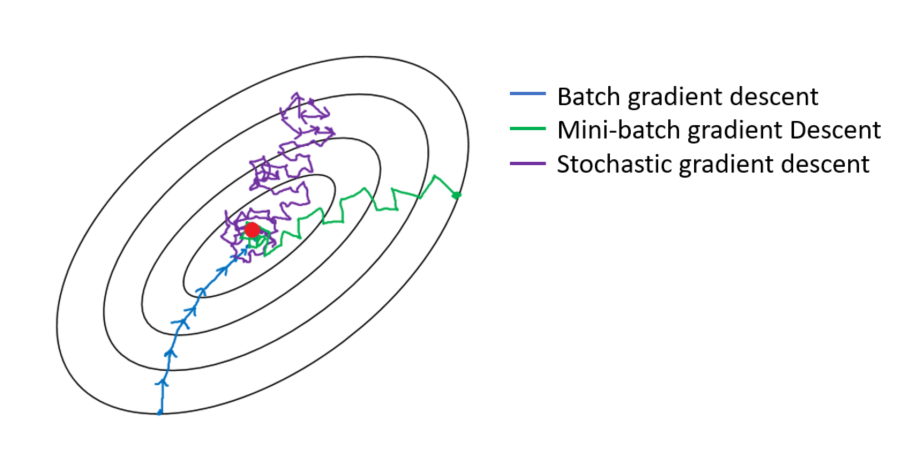
\includegraphics[scale=0.3]{img}
\end{figure}

\subsection{Extensions}

The basic SGD algorithm has been extended in many different ways. The popularity of
the algorithm disallows a comprehensive or detailed treatment of all
developments. This sub-section covers some of the more important and interesting
ones.


\subsubsection{Step Size}

As hinted at in our proof of convergence to $\hat{w}$, much depends on
an appropriately chosen step size $\gamma$. If $\gamma$ is too small, gradient
descent may
take an excessively long time to run (since we are only moving a small distance
``down'' the gradient every iteration); if $\gamma$ is too large, then an
iteration's step may ``overshoot'' the critical point.
An entire literature has developed around the best way to select $\gamma$. The
central insight that is common to most $\gamma$-selection methods is to treat it
as a time-indexed rather than fixed hyperparameter, i.e., $\gamma^{(t)}$ rather
than $\gamma$. Ideally we would like $\gamma^{(t)}$ to be large when far away
from the critical point (so as to increase speed of convergence) and to be small
when close to the critical point (so as to avoid overshooting).

Line search is one method for computing step size. As described in
\cite{boyd2004convex}, there are two main variants: \textit{exact} and
\textit{backtracking}. In exact line search, $\gamma^{(t)}$ is chosen to minimize $f$
along the ray $\{x + \gamma^{(t)} \Delta x\}$, where $\gamma^{(t)} \in \mathbb{R}^+)$ and
$\Delta x$ is the descent direction determined by SGD:
\begin{equation}
	\gamma^{(t)} = \argmin_{s \geq 0} f(x + s\Delta x)
\end{equation}
This obviously is an optimization problem in and of itself, and
so it can be computationally impractical to add this burden in addition to the
``main'' optimization problem we are trying to solve using SGD. For this reason,
\textit{backtracking} is an iterative approximation method that is
computationally lighter. The backtracking algorithm takes two hyper-parameters
$\alpha \in (0, 0.5)$ and $\beta \in (0, 1)$. It starts with an initial guess of
$s^{(0)} = 1$, and then for every iteration $t$, updates $s := \beta t$. The
algorithm stops when $f(x + s \Delta x) \leq f(x) + \alpha s \Delta f(x)^T
\Delta x$, and the final value of $s$ is taken as $\gamma^{(t)}$. 

\cite{bottou2012stochastic} advocates using learning rates of the form
$\gamma^{(t)} = \gamma^{(0)}(1 + \gamma^{(0)}\lambda t)^{-1}$. When the Hessian
$H$ of $f$ is strictly positive, using $\gamma^{(t)} =
(\lambda_{\mathrm{min}}t)^{-1}$, where $\lambda_{\mathrm{min}}$ is the smallest
eigenvalue of $H$, produces the best convergence speed. Note that $
(\lambda_{\mathrm{min}}t)^{-1}$ decreases asymptotically with $t$, matching our intuition
about larger step sizes in early iterations and smaller step sizes in later
iterations. However, simply using $\gamma^{(t)} =
(\lambda_{\mathrm{min}}t)^{-1}$ can produce \textit{too} large of steps in early
iterations. Hence, it often works better to start with some reasonable initial
estimate $\gamma^{(0)}$ that then decays in the fashion of
$(\lambda_{\mathrm{min}}t)^{-1}$, leading to the expression in the first
sentence of this paragraph. By definition, ``reasonable'' is more of a judgment
call than a mathematical statement: Bottou provides some heuristics for creating
such an estimate of $\gamma^{(0)}$.

\subsubsection{Momentum and Acceleration}

In our set-up of SGD, we stipulated that the function to be minimized, $f$, is
convex. Although this is a necessary condition for some proofs of SGD's
correctness, SGD is widely used in applications---most prominently, neural
networks and deep
learning---where this assumption is not
always true. In such settings, it is
possible that there are multiple local minima, and/or that there are areas where
the surface curves much more steeply in one dimension than another. The challenge for SGD is
how to avoid getting ``stuck'' in these local ravines and continue iterating
until the true global minimum is achieved. Even if there is no pathological
curvature, incorporating information about the local topology may result in more
efficient algorithms and faster convergence.

Momentum---also called acceleration---is a common modification of GD. As outlined in
\cite{rumelhart1986general} and 
\cite{qian1999momentum}, we add a new acceleration term to the familiar GD
equation. Let $z^{(t+1)} = \alpha z^{(t)} + \nabla f(w^{(t)})$. GD with
momentum then is:

\begin{equation}
	w^{(t+1)} = w^{(t)} - \gamma z^{(t+1)}
\end{equation}

Now, the weight vector obtained for the current timestep depends both on the
current gradient \textit{and the update of the previous time-step}, with the
acceleration parameter $\alpha$ governing how much weight is given to the
previous time-step. 
This formulation leads to momentum: dimensions whose
gradients point in the same direction have proportionally greater updates, while
dimensions whose gradients exhibit strong curvature have proportionally
lesser updates. The effect is to help stop (S)GD from oscillating in ravines and
speed up convergence. There are many variations on acceleration, including
Nesterov accelerated gradient (NAG) (\cite{nesterov}), Adam
(\cite{kingma2014adam}), AdaGrad
(\cite{duchi2011adaptive}), and AdaDelta (\cite{zeiler2012adadelta}).

\subsubsection{Averaging}

Averaged SGD (ASGD)---to the author's knowledge first proposed in 
\cite{polyak1992acceleration}---is another variation. Typically, we consider
$\hat{w}$ (the optimal solution) to be that associated with the final iteration
of SGD, when some stop condition is met. For example, in a situation where we
run $N$ iterations before stopping, $\hat{w} = w^{(N)}$. In ASGD, we consider $\hat{w}$ 
the average of $w$ across all iterations, i.e.
\begin{equation}
	\hat{w} = \bar{w} = \frac{1}{N} \sum_{t=1}^N w^{(t)}
\end{equation}

The value proposition of ASGD is that sometimes SGD will oscillate around the
optimal solution. By taking the average across all updates, ASGD reduces this
noise and is likely to give a solution closer to the optimum. More sophisticated
versions of ASGD have been proposed in 
\cite{zhang2004solving}
and 
\cite{xu2011towards}. 

\subsubsection{Mini-batch}

Mini-batch gradient descent (MGD) can be regarded as a mid-point between batch
and stochastic gradient descent in that it uses more than one but less than all of
the available observations. Suppose we have $n$ observations and divide them
into $m$ groups called mini-batches, each of equal size $b=\frac{n}{m}$. Now, at
every iteration $t$, randomly pick one of the mini-batches (all are equally
likely to be chosen). For that mini-batch:

\begin{equation}
	w^{(t+1)} = w^{(t)} - \gamma \frac{1}{b} \sum_{i=1}^b \nabla f(w^{(t)})
\end{equation}

MGD iterates with $t$ and converges to $\hat{w}$ in the normal manner. Every
update, a new $b$ is randomly chosen and the above algorithm iterated. 
\cite{dekel2012optimal} and \cite{li2014efficient} analyze MGD's speed of
convergence and suggest that has some advantageous qualities for
parallelization, a topic that is explained in more depth in the following
subsection.

\subsubsection{Parallelization}

SGD is commonly used in large-$n$ applications. Thus,
even though SGD is a computational improvement over batch GD, there has been
interest in whether SGD can be made even faster by parallelizing it. As
background, typical computer applications are serial: problems are broken
down into a discrete series of instructions that are executed one after another
on a single processor. Parallel computing calls for breaking down problems into discrete parts that can
be solved concurrently and are executed simultaneously on multiple processors
(\cite{barney2010introduction}).
There are many paradigms of parallel computing but a useful high-level
distinction is between shared memory, in which all processors share a common
address space, and distributed memory, in which each processor or group of processors
has its own address space. The latter has become increasingly popular in
industry via Apache Hadoop and associated projects (e.g. Spark). Distributed
memory applications often require very complex computing strategies for how to combine the
work of many processors without a shared memory space into a single coherent answer.

This background helps to emphasize the novelty of the parallel
implementation of SGD proposed in \cite{zinkevich2010parallelized}. Though backed
by highly technical proofs, the actual algorithm is strikingly simple. Suppose we have $N$ processors. We seek to
conduct SGD to estimate $w$ across $n$ observations with fixed learning rate
$\gamma$ for some fixed number of steps $T$.

\medskip

\begin{algorithm}[H]
	Define $T = \frac{n}{N}$\;

	Randomly partition examples, giving $T$ to each machine;\

	\ForAll{$i \in \{1 \ldots N\}$}{
		Randomly shuffle data on machine $i$\;

		Initialize $w^{i, (0)}=0$\;

		\ForAll{$t \in \{1 \ldots T\}$}{
			
	$w^{i, (t+1)} = w^{i, (t)} - \gamma \nabla f(w^{i, (t)})$ \;
			}
		}
	Aggregate from all computers: $\bar{w} = \frac{1}{N} \sum_{i=1}^{N}
	w^{i, (T)}$ \;

	\Return{$\bar{w}$}

	\caption{Parallel SGD}
\end{algorithm}

\medskip

Zinkevich et al. show that this algorithm has a number of desirable properties.
It requires no communication between machines until the end; asymptotically, the
error approaches zero; and, the amount of time required is independent of the number of
examples (though this is an inherent property of SGD and is not unique to their
algorithm). Further improvements have been proposed: e.g., the Hogwild algorithm
presented in \cite{recht2011hogwild} deals with locking issues in parallel
computation of SGD.

\section{Applications}

In theory, SGD is agnostic to $f$ and $w$ as long as they meet required
assumptions, and so can be used in many different areas of optimization. In
practice, SGD is overwhelmingly popular in the statistical learning
field for estimating weight coefficients in predictive models. 
This section lays out some reasons for SGD's popularity; conducts a case study
using SGD; and identifies notable real-world applications of SGD. 

\subsection{SGD and Statistical Learning}
\cite{shalev2011pegasos}

Loosely following the set-up of , consider a typical supervised classification problem. We have
feature matrix $\bm{X}_{n \times D, n \in \mathbb{R}^n, D \in \mathbb{R}^D}$ (corresponding to $n$ observations and $D$
features) and labels $\bm{Y}_{n \times 1}, Y_i \in \{-1, 1\}$. The goal is to
predict a particular observation's label $Y_i$ using that observation's features $\bm{X}_i$. 
We have a hypothesis class $\mathcal{F}$ consisting of
various functions $f_{\bm{w}}(\bm{X}_i) \in \mathcal{F}$ parametrized by weight
vector $\bm{w}$. We have loss function $L(Y_i, f_{\bm{w}}(\bm{X}_i))$ that
expresses the cost of mis-classification. Assume for now that $L$ is convex. 
We will consider the optimal function $\hat{f}_{\bm{w}}(\bm{X}_i) \in F$ 
that which minimizes empirical risk over all observations: $\frac{1}{n}
\sum_{i=1}^n L(Y_i, f_{\bm{w}}(\bm{X}_i))$.
Denote $\hat{\bm{w}}$ the weight coefficients of this optimal function. We thus
have:

\begin{equation}
	\hat{\bm{w}} = \argmin_{\bm{w}}\frac{1}{n} \sum_{i=1}^n L(Y_i, f_{\bm{w}}(\bm{X}_i))
\end{equation}

Because $L$ is convex, there is one critical point,
it is the global minimum, and it is located where the gradient of the loss
function with respect to $\bm{w}$ is zero. GD is an iterative
algorithm that can be used to numerically approximate this point. We first state
it in a general form, and then adapt it to the specific problem outlined above.

\begin{equation}
	\bm{w}_{t+1} = \bm{w}_t - \gamma \frac{1}{n}\sum_{i=1}^n
	\nabla L(Y_i, f_{\bm{w}_t}(\bm{X}_i))
\end{equation}

$t$ refers to iterations. $\gamma$ is a parameter controlling the step
size (also called ``learning rate''). Assume for now that $\gamma$ is fixed. For
$t=0$ we must supply an initial starting guess, $\bm{w}_0$.  

\begin{equation}
	\left|\frac{1}{n}\sum_{i=1}^n \nabla L(\bm{Y}_i,
	f_{\bm{w}_t}(\bm{X}_i))\right| \leq \epsilon
\end{equation}

Note that the batch GD algorithm presented in (2) requires evaluating the
gradient for every single observation $i$. In a large-$n$ dataset, this can be
computationally infeasible. SGD's innovation is to instead evaluate only a
single randomly chosen observation $i$ at each iteration $t$.

\begin{equation}
	\bm{w}_{t+1} = \bm{w}_t - \gamma 
	\nabla L(Y_i, f_{\bm{w}_t}(\bm{X}_i))
\end{equation}

\subsection{Case Study}

\cite{dal2015calibrating}

\subsection{Real-World Applications}

If a Silicon Valley press release uses words like ``artificial intelligence'',
``machine learning'', and ``big data'' to describe a new product or service, it very likely
uses SGD in some way. Such is the extent of SGD's popularity. 
Below is a list of particularly prominent examples of SGD's practical
applications.

\begin{itemize}
	\item \textbf{ImageNet} is a dataset consisting of millions
		of high-resolution, labeled images. The
		ImageNet Large Scale Visual Recognition Competition (ILSVRC) is
		an annual contest in which competing teams train models for
		automatic image classification. The submission of \cite{krizhevsky2012imagenet} 
		for the 2012 ILSVRC used convolutional neural
		nets to achieve dramatic reduction in error rates and is
		one of the most cited machine learning papers of all time. Per the aforementioned paper: ``We
		trained our models using stochastic gradient descent with a
		batch size of 128 examples, momentum of 0.9, and weight decay of
		0.00005.''
	\item Google's \textbf{AlphaGo} software. AlphoGo applies deep learning to the
		board game of Go and has received extensive attention for its
		ability to defeat even top human players (e.g., twice making the
		cover of \textit{Nature} with \cite{silver2016mastering} and
		\cite{silver2017mastering}). Google's slides from the 2016
		International Conference on Machine Learning (ICML) indicate
		that SGD is used in every stage of the
		model: supervised learning of policy networks, reinforcement
		learning of policy networks, and reinforcement learning of value
		networks.
	\item The \textbf{Netflix Grand Prize} was a competition hosted by
		Netflix in which teams competed to develop models for
		using Netflix data to make better movie recommendations
		(\cite{bennett2007netflix}). Most of the top entries used
		SGD for estimating model coefficients; for example,
		\cite{koren2009bellkor} states that ``in order to learn the
		involved parameters$\ldots$ learning is done by a stochastic
		gradient descent algorithm running for 30 iterations.'' 
	\item Google's \textbf{word2vec} natural language processing (NLP)
		software powers Google Translate, among other applications.
		\cite{mikolov2013distributed} and \cite{rong2014word2vec}
		discuss the continuous bag of words (CBOW) model underlying
		word2vec and how SGD is used to estimate coefficients
		in the model.
\end{itemize}

\section{Conclusion}

\printbibliography

\end{document}


